\begin{frame}{Introduction}
	The Capacitated Vehicle Routing Problem (\textbf{CVRP}) \parencite{dantzig1959}
	is an \textcolor{blue}{NP-hard combinatorial optimization routing problem} with applications in \textcolor{blue}{logistics}, such as delivery of goods or services to customers.

	\vspace{0.3cm}

	\begin{columns}
		\begin{column}{.35\textwidth}
			\centering
			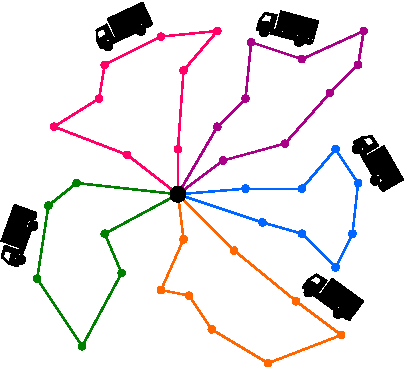
\includegraphics[height=4cm]{Imgs/CVRP-example.cropped.pdf}
		\end{column}
		\begin{column}{.65\textwidth}
			CVRP defined on an undirected graph. We are given:
			\begin{itemize}
				\item A \textcolor{blue}{central depot node}.
				\item Nodes' \textcolor{blue}{locations}.
				\item The \textcolor{blue}{demands} of the individual customers.
				\item The amount of \textcolor{blue}{available vehicles} with their \textcolor{blue}{capacity}.
			\end{itemize}
			Objective:
			\begin{itemize}
				\item \textcolor{red}{Minimize overall routing costs while meeting the needs of \textbf{all} customers.}
			\end{itemize}
		\end{column}
	\end{columns}

\end{frame}

\begin{frame}{Branch-price-and-cut}
	\begin{columns}
		\begin{column}{.8\textwidth}

			\begin{itemize}
				\item \textcolor{blue}{Branch-price-and-cut}: is an \textbf{exact approach} for solving combinatorial optimization problems. It is an extension of traditional \textcolor{blue}{branch-and-cut} (BAC) frameworks.
				      \begin{itemize}
					      \item State-of-the-art in VRPs.
				      \end{itemize}
				\item Compared to traditional BAC frameworks, can tackle huge \textcolor{blue}{mixed integer programming models} described by exponential amounts of decision variables.
				\item \textcolor{red}{How?}
				      \begin{itemize}
					      \item \textcolor{blue}{Column Generation} (CG): decision variables are generated lazily in an attempt to improve the dual bounds and reach optimality.
					      \item \textcolor{red}{Pricing} is the art of producing decision variables for the BPC approach to evolve.
					      \item In VRP, decision variables represent \textcolor{blue}{single vehicle feasible routes}.
				      \end{itemize}
			\end{itemize}
		\end{column}
		\begin{column}{.2\textwidth}
			\begin{tiny}
				\begin{align*}
					\min_{\lambda} \quad z_\mt{SC}(\lambda) & = \sum_{p \in P}  c_p \lambda_p                                      \\
					                                        & \sum_{p \in P} \lambda_{p} = K                                       \\
					                                        & \sum_{p \in P}  a_{ip} \lambda_p \ge 1       \quad \forall i \in V_0 \\
					                                        & \lambda_p                    \in \Set*{0, 1} \quad \forall p \in P.
				\end{align*}
			\end{tiny}
		\end{column}

	\end{columns}
\end{frame}

\begin{frame}{The Pricing Sub-problem}
	To advance the column generation, the \textcolor{blue}{pricer}, a critical component in BPC frameworks, needs to solve the \textcolor{blue}{pricing sub-problem} (PP):
	\begin{itemize}
		\item An \textcolor{blue}{Elementary Shortest Path Problem with Capacity Constraints} (\textbf{ESPPCC}) in a reduced cost network with negative cycles.
		      \begin{itemize}
			      \item NP-hard problem \parencite{dror1994}.
		      \end{itemize}
		\item \textbf{Relax elementarity condition} to make it solvable in pseudo-polynomial time:
		      \begin{itemize}
			      \item $q$-routes with 2-cycles elimination \parencite{christofides1969}.
			      \item $q$-routes with arbitrary $k$-cycles elimination \parencite{christofides1969}.
			      \item ng-routes \parencite{baldacci2011}.
		      \end{itemize}
		\item State-of-the-art solutions for the \textcolor{red}{relaxed} PP are based on \textcolor{blue}{dynamic programming}:
		      \begin{itemize}
			      \item \textbf{labeling algorithm} \parencite{desrochers1992, feillet2004}.
		      \end{itemize}
	\end{itemize}
\end{frame}

\begin{frame}{Thesis Contributions}
\end{frame}

\begin{frame}{Implementation}
\end{frame}

\begin{frame}{Empirical evaluation}
	\begin{itemize}
		\item Running time measured through \textbf{performance profiles} \parencite{dolan2002}.
	\end{itemize}
\end{frame}

\begin{frame}{Results (1/2)}

\end{frame}

\begin{frame}{Results (2/2)}

\end{frame}

\begin{frame}{Conclusions and Future Work}
	\cite{jepsen2014}
\end{frame}

\begin{frame}{The end}
	\begin{center}
		\begingroup
		\fontsize{18pt}{18pt}\selectfont
		Thank, you.
		\endgroup
	\end{center}
\end{frame}

\appendix

\begin{frame}
\end{frame}

\begin{frame}
	\begin{center}
		\begingroup
		\fontsize{18pt}{18pt}\selectfont
		Appendix.
		\endgroup
	\end{center}
\end{frame}

\begin{frame}{Integer Programming}
	MIP solvers are rather general and can be used to solve a wide range of problems from various fields \parencite{bixby2007progress}.
	MIP models are, in spirit, a way to mathematically program a solver to achieve the desired solution.
	A MIP solver can solve a mixed-integer linear programming formulation
	expressed as \parencite{wolsey1999integer}:
	\begin{align}
		 & \max_{x, y} & c^T x + d^T y                                 \\
		 & \text{s.t.} & A x + B y \le b  \label{eq:general-mip-bound} \\
		 &             & x \in \R^n                                    \\
		 &             & y \in \Z_{+}^k,
	\end{align}
	where $A \in \R^{m \times n}, B \in \R^{m \times k}$ are matrices and
	$c \in \R^n, d \in R^k, b \in \R^m$ are vector coefficients.
	The bound in \cref{eq:general-mip-bound} can also be rewritten in equality and/or greater form.

\end{frame}

\begin{frame}{Set Covering formulation}
	Let $P = \Set*{p \mid p\ \text{is a single-truck elementary feasible route}}$ be the set of all feasible routes.

	\begin{align}
		\min_{\lambda} \quad z_\mt{SC}(\lambda) & = \sum_{p \in P}  c_p \lambda_p              & \label{eq:set-covering-obj-func}                                                       \\
		                                        & \sum_{p \in P} \lambda_{p} = K               & \label{eq:set-covering-K-routes}                                                       \\
		                                        & \sum_{p \in P}  a_{ip} \lambda_p \ge 1       & \quad \forall i \in V_0 \label{eq:set-covering-customers-visited-by-exactly-one-route} \\
		                                        & \lambda_p                    \in \Set*{0, 1} & \quad \forall p \in P \label{eq:set-covering-lambda-mip-var-bounds}.
	\end{align}
\end{frame}
